\documentclass[10pt]{standalone}
\usepackage{amsmath}
\usepackage{amsthm}
\usepackage{tikz}
\usetikzlibrary{calc}
\usetikzlibrary{shapes,arrows,positioning}
\tikzstyle{decision} = [diamond, draw, 
    text width=6em, text badly centered, node distance=3cm, inner sep=0pt]
\tikzstyle{block} = [rectangle, draw,
    text width=9em, text centered, rounded corners, minimum height=4em]
\tikzstyle{line} = [draw, -latex']
\tikzstyle{cloud} = [draw, ellipse,fill=red!20, node distance=3cm,
    minimum height=2em]

%% END MACROS SECTION


\begin{document}

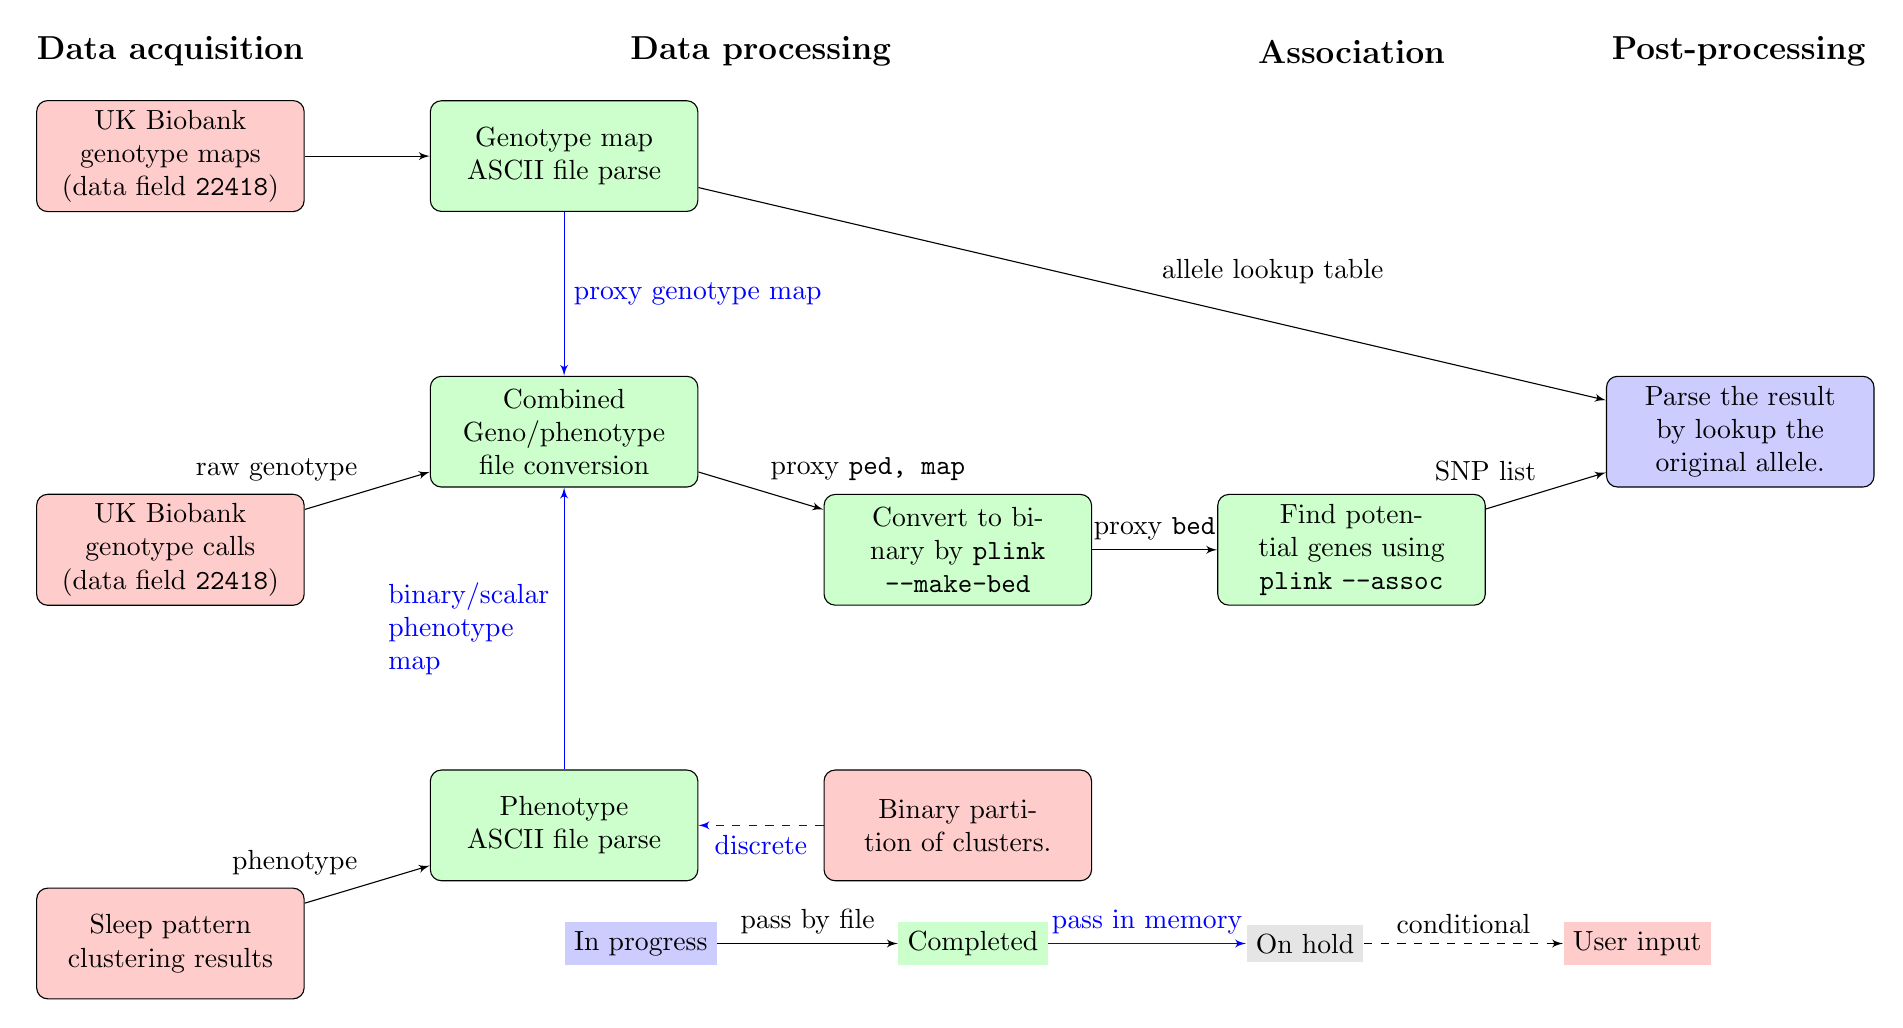
\begin{tikzpicture}[node distance = 5cm, auto]
\node[block,fill=red!20](DA_G_map){UK Biobank genotype maps (data field \texttt{22418})};
\node[block,fill=red!20, below of = DA_G_map ](DA_G_raw){UK Biobank genotype calls (data field \texttt{22418})};
\node (aux_DA_up) at($(DA_G_map)!0.7!(DA_G_raw)$) {};
\node[block,fill=red!20,below of = DA_G_raw](DA_P){Sleep pattern clustering results};
\node (aux_DA_down) at($(DA_G_raw)!0.7!(DA_P)$) {};
\node[block,right of = DA_G_map,fill=green!20](DP_G_mformat){Genotype map ASCII file parse};
\node[block,right of = aux_DA_up,fill=green!20](DP_G_format){Combined Geno/phenotype file conversion};
\node[block,right of = aux_DA_down,fill=green!20](DP_P_format){Phenotype ASCII file parse};
\node[block, right of = DP_P_format,fill=red!20](DP_partition_input){Binary partition of clusters.};
\path(DA_G_map)edge[line] node (DA_G_mp){}(DP_G_mformat);
%\path(DA_G_map)edge[line,dashed] node(DA_G_UKB_DP_p){genotype}(DP_G_format);
\path(DA_G_raw)edge[line] node(DA_G_UKB_DP_p){raw genotype}(DP_G_format);
\path(DA_P)edge[line] node(DA_P_DP_p){phenotype}(DP_P_format);
\node (aux_DP) at($(DP_G_format)!0.3!(DP_P_format)$) {};
\node[block,fill=green!20,right of = aux_DP](DP_C){Convert to binary by \texttt{plink --make-bed}};
\node (aux_DPC) at($(aux_DP)!0.5!(DP_C)$) {};
\path(DP_G_format)edge[line]node(DP_G2C){proxy \texttt{ped, map}}(DP_C);
\path(DP_P_format)edge[line,color=blue]node[text width = 6em](DP_P2G){binary/scalar phenotype map}(DP_G_format);
\path(DP_partition_input)edge[line,color=blue,dashed]node(DP_partition_to_parse){discrete}(DP_P_format);
\node[block,fill=green!20,right of = DP_C] (AS) {Find potential genes using \texttt{plink --assoc}};
\path(DP_C)edge[line]node(DP_C_2_AS){proxy \texttt{bed}}(AS);
\node[block,fill=blue!20, right of = DP_G_format, node distance = 42.5em] (PP_G) {Parse the result by lookup the original allele.};
\path(AS)edge[line]node(AS_2_PP_G){SNP list}(PP_G);
\path(DP_G_mformat)edge[line]node(DP_G_LUT_PP){allele lookup table} (PP_G);
\path(DP_G_mformat)edge[line,color=blue]node(DP_G_m2r){proxy genotype map}(DP_G_format);
%Titles: 
\node[above of = DA_G_raw,node distance = 18em](DA_t){\large \textbf{Data acquisition}};
\node[above of = aux_DPC,node distance = 18em](DA_t){\large \textbf{Data processing}};
\node[above of = AS,node distance = 18em](DA_t){\large \textbf{Association}};
\node[right of = DA_t, node distance = 14em](PP_t){\large \textbf{Post-processing}};
%Legends:
\node[right of = DA_P,node distance = 17em,fill=blue!20](L_ip){In progress};
\node[right of = L_ip,node distance = 12em, fill=green!20](L_C){Completed};
\node[right of = L_C,node distance = 12em, fill=gray!20](L_H){On hold};
\node[right of = L_H, node distance = 12em, fill=red!20](L_U){User input};
\path(L_ip)edge[line,color=black]node(L_file_pass){pass by file}(L_C);
\path(L_C)edge[line,color=blue]node(L_mem_pass){pass in memory}(L_H);
\path(L_H)edge[line,dashed]node(L_mem_pass){conditional}(L_U);

%\node[block,fill=blue!20,right of = R_2_M](M_OB){Set a scalar oberservation function that measures sleep on a continuous scale};
%\path(R_2_M)edge[line](M_OB);
%\node[below of = R_DA,node distance = 4cm, block,fill=blue!20](M_Framework){Set simulation framework for using Bayesian filter(past work)};
%\node[decision,below of = M_OB,node distance = 4cm, fill=blue!20](M_FIT){Find most probable parameter that matches observation};
%\node(M_Model)[below of = R_2_M,node distance = 4cm, block,fill=blue!20]{Pick oscillator model (discussed last week)};
%\path(M_Framework) edge[line]node[midway]{}(M_Model);
%\path(M_Model) edge[line]node[midway]{}(M_FIT);
%\path(M_FIT) edge[line,dotted,out=150,in=30]node[midway]{poor fit}(M_Model);
%\path(M_OB) edge[line] node [midway,left]{observation in $r$}(M_FIT);
%\node[block,right of=M_FIT,node distance = 6cm,fill=blue!20](E_P){Improve classification (partial progress)};
%\path(M_FIT) edge[line,dotted]node[midway]{reliable prediction}(E_P);
%\node[block,below of=M_FIT,node distance = 4cm,fill=red!20](E_C){Relate difference in parameter to difference in experiment setup (limited reliability)};
%\path(M_FIT)edge[line,dotted]node [midway,left]{compare parameter}(E_C);
%\node[block](VY){$V_Y$, wake undisturbed};
%\node[block, right of=VY, node distance = 8cm](VV){$V_V$};
%\node[block, below of=VV, node distance = 3cm](KV){$K_V$ (slow,decay)};
%\path(VY)edge[line,out=45,in=135]node [midway]{$+\beta \phi(V_Y)$} (VV);
%\path(VV)edge[line,out=215,in=305]node [midway]{$-\alpha\phi(V_V)$} (VY);
%\path(VY)edge[line,out=135,in=225,loop]node [midway,left]{$+\beta\phi(V_Y)$} (VY);
%\path(KV)edge[line,out=135,in=215] node[midway,left]{$+$}(VV);
%\path(VV)edge[blue,line,out=305,in=45] node[midway,right]{$+$,accumulative}(KV);
%\path(VY)edge[blue,line,out=305,in=135] node[midway,above]{$+$,accumulative}(KV);
%\node[above left of=VY,node distance = 2.5cm](rectY-refA){};
%\node[below right of=VY,node distance = 2.5cm](rectY-refB){};
%\draw [red,thick,dotted](rectY-refA)  rectangle node[black,below=2cm]{pyramidal neurons} (rectY-refB);
%\node[above left of=VV,node distance = 2.5cm](rectV-refA){};
%\node[below right of=KV,node distance = 2.5cm](rectV-refB){};
%\draw [red,thick,dotted](rectV-refA)  rectangle node[black,below=3.5cm]{PV neurons} (rectV-refB);
\end{tikzpicture}


\end{document}